\PassOptionsToPackage{table}{xcolor}
\documentclass{article}

\usepackage[utf8]{inputenc}
\usepackage[T1]{fontenc}
\usepackage{color}

\usepackage[english]{babel}

\usepackage[margin=1in]{geometry}  % set the margins to 1in on all sides
\usepackage{graphicx}              % to include figures
\usepackage{amsmath}               % great math stuff
\usepackage{amsfonts}              % for blackboard bold, etc
\usepackage{amsthm}                % better theorem environments
\usepackage{enumerate}

\usepackage{tikz}
\usepackage{colortbl}
\usepackage[table]{xcolor} 

\usepackage{hyperref}
\usepackage{listings}
\usepackage{subcaption}
\usepackage{placeins}
\usepackage{fancyref}

\usepackage{fancyhdr} % Required for custom headers
\usepackage{lastpage} % Required to determine the last page for the footer
\usepackage{extramarks} % Required for headers and footers

\usepackage{todonotes}
\usepackage{float}
\usepackage[noend, boxruled, linesnumbered]{algorithm2e}

\usepackage[parfill]{parskip}

% Set up the header and footer

\renewcommand\headrulewidth{0.4pt} % Size of the header rule
\renewcommand\footrulewidth{0.4pt} % Size of the footer rule

\setlength\parindent{0pt} % Removes all indentation from paragraphs
\setlength{\parskip}{8pt}

\lstdefinestyle{customc}{
  belowcaptionskip=1\baselineskip,
  breaklines=true,
  language=C++,
  showstringspaces=false,
  basicstyle=\small\ttfamily,
  keywordstyle=\bfseries\color{green!40!black},
  commentstyle=\itshape\color{purple!40!black},
  identifierstyle=\color{blue},
  stringstyle=\color{orange},
  numbers=left,                    % where to put the line-numbers; possible values are (none, left, right)
  numbersep=5pt                   % how far the line-numbers are from the code
}
\lstset{escapechar=@,style=customc}

\newcommand{\xor}{\oplus}
\newcommand{\myo}{\mathcal{O}}
\newcommand{\myb}{\mathcal{B}}

\newcommand{\illustrate}[2]{
  \begin{center}
    
\includegraphics[page=#1,width=#2\textwidth]{graphics/illustrations}
  \end{center}
}


%%% Local Variables:
%%% mode: latex
%%% TeX-master: "main"
%%% End:


\author{The author 1\\The author 2}
\title{This is the title}

\begin{document}
\maketitle

\tableofcontents
\newpage


\section{First section}
\label{sec:first-section}

This is the first section. This section contains stuff like

\begin{itemize}
\item Items
\item and more
\item items
\end{itemize}

You could also

\begin{enumerate}
\item Enumerate
\item Them
\end{enumerate}

or make descriptions:
\begin{description}
\item[This:] is a description
\item[Where:] things are described
\end{description}

\section{Figures}
\label{sec:figures}

This section includes some figures and tables. Note that a
\texttt{$\backslash$FloatBarrier} draws a line in the sand
and keeps the figure from floating passed it.

\begin{figure}
  \centering
  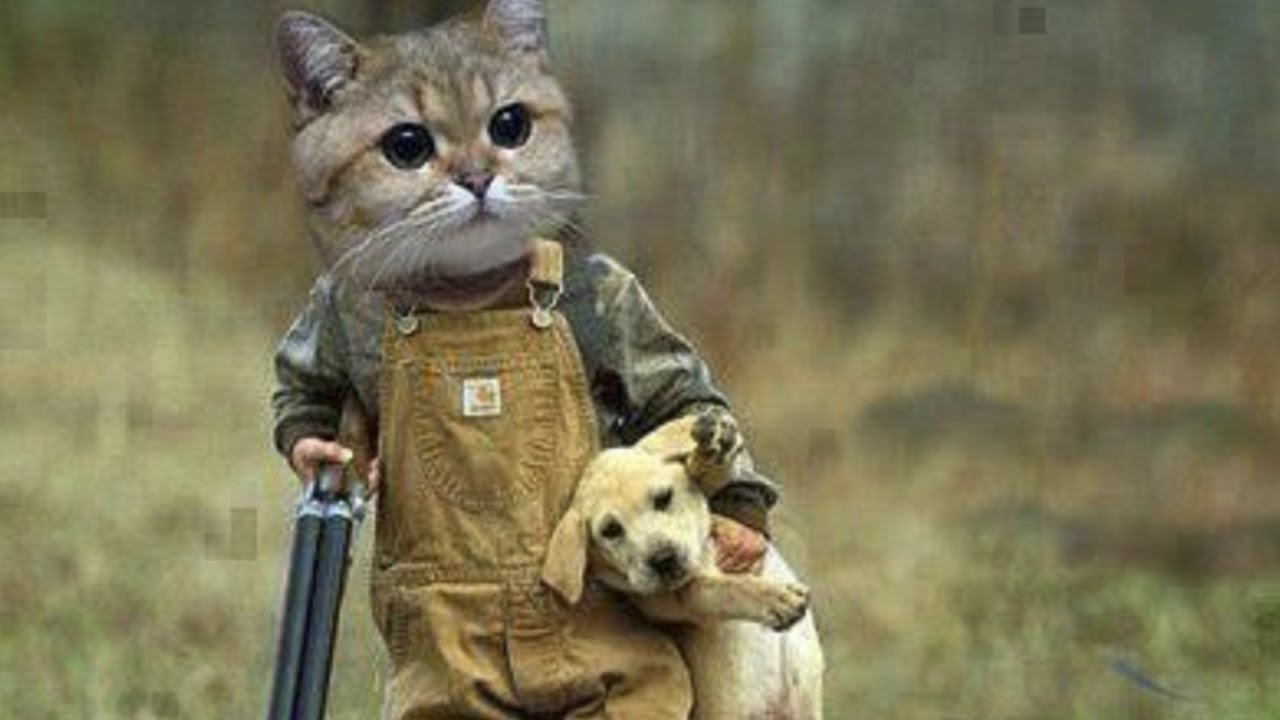
\includegraphics[width=0.6\textwidth]{graphics/cat1}
  \caption{Cat number one.}
  \label{fig:cat1}
\end{figure}


\begin{figure}
  \centering
  
\includegraphics[width=0.6\textwidth]{graphics/cat2}
  \caption{Cat number 2}
  \label{fig:cat2}
\end{figure}

\begin{figure}[h!]
  \centering
  \illustrate{1}{0.3}
  \caption{Imported from graphics/illustrations.pdf using
    simple macro}
  \label{fig:import}
\end{figure}

\FloatBarrier

\section{References}
\label{sec:references}

This is a section that references to the others. For instance one can
see \Fref{fig:cat1} - or we can reference to a section number
\ref{sec:figures} like that. You can also reference an \Fref{eq:roots}
or Table \ref{tab:greek-letters}

\section{This section is included from another file}
\label{sec:included-section}

In this section we present a short table of greek letters. And a bit
of math:

\begin{equation}
  \label{eq:roots}
  x = \frac{-b \pm \sqrt{d}}{2a}
\end{equation}

Or math that doesn't need referencing:

$$
a^2 + b^2 = c^2
$$

\begin{table}[h]
  \centering
  \begin{tabular}{c l c l}
    \textbf{Greek letters} & \textbf{In \LaTeX} & \textbf{Other symbold} &
                                                             \textbf{In \LaTeX}\\
    $\alpha$ & \textbackslash alpha & $\{$ & \textbackslash \{ \\
    $\beta$ & \textbackslash beta & $\}$ & \textbackslash \} \\
    $\gamma$ & \textbackslash gamma & $\dots$ & \textbackslash dots \\
    $\epsilon$ & \textbackslash epsilon & $\leq$ & \textbackslash leq \\
    $\varepsilon$ & \textbackslash varepsilon & $\geq$ &
                                                         \textbackslash geq \\
    $\zeta$ & \textbackslash zeta & $\rightarrow$ & \textbackslash rightarrow \\
    $\eta$ & \textbackslash eta & $\Rightarrow$ & \textbackslash Rightarrow \\
    $\theta$ & \textbackslash theta & $\wedge$ & \textbackslash wedge \\
    $\gamma$ & \textbackslash gamma & $\vee$ & \textbackslash vee \\
    $\lambda$ & \textbackslash lambda & $\vdots$ & \textbackslash vdots \\
    $\mu$ & \textbackslash mu & $\otimes$ & \textbackslash otimes \\
    $\nu$ & \textbackslash nu & $\cdot$ & \textbackslash cdot \\
    $\xi$ & \textbackslash xi & $\bigcup$ & \textbackslash bigcup \\
    $\pi$ & \textbackslash pi & $\bigcap$ & \textbackslash bigcap \\
    $\rho$ & \textbackslash rho & $\pm$ & \textbackslash pm \\
    $\sigma$ & \textbackslash sigma & & \\
    $\tau$ & \textbackslash tau & & \\
    $\phi$ & \textbackslash phi & & \\
    $\chi$ & \textbackslash chi & & \\
    $\Delta$ & \textbackslash Delta & & \\
    $\Theta$ & \textbackslash Theta & & \\
    $\Omega$ & \textbackslash Omega & &
  \end{tabular}
  \caption{Greek letters - Remember math mode}
  \label{tab:greek-letters}
\end{table}

%%% Local Variables:
%%% mode: latex
%%% TeX-master: "main"
%%% End:



\end{document}

%%% Local Variables:
%%% mode: latex
%%% TeX-master: t
%%% End:
